%% LaTeX Template for ISIT 2025
%%
%% by Stefan M. Moser, October 2017
%% (with minor modifications by Tobias Koch, November 2023 and Michèle Wigger, November 2024)
%% 
%% derived from bare_conf.tex, V1.4a, 2014/09/17, by Michael Shell
%% for use with IEEEtran.cls version 1.8b or later
%%
%% Support sites for IEEEtran.cls:
%%
%% http://www.michaelshell.org/tex/ieeetran/
%% http://moser-isi.ethz.ch/manuals.html#eqlatex
%% http://www.ctan.org/tex-archive/macros/latex/contrib/IEEEtran/
%%


\documentclass[conference,letterpaper]{IEEEtran}


%% depending on your installation, you may wish to adjust the top margin:
\addtolength{\topmargin}{9mm}
\textheight 9.34in

%%%%%%
%% Packages:
%% Some useful packages (and compatibility issues with the IEEE format)
%% are pointed out at the very end of this template source file (they are 
%% taken verbatim out of bare_conf.tex by Michael Shell).
%
% *** Do not adjust lengths that control margins, column widths, etc. ***
% *** Do not use packages that alter fonts (such as pslatex).         ***
%
\usepackage[utf8]{inputenc} 
\usepackage[T1]{fontenc}
\usepackage{url}
\usepackage{ifthen}
\usepackage{cite}
\usepackage{comment}
\usepackage[cmex10]{amsmath} % Use the [cmex10] option to ensure complicance
                             % with IEEE Xplore (see bare_conf.tex)
%% Please note that the amsthm package must not be loaded with
%% IEEEtran.cls because IEEEtran provides its own versions of
%% theorems. Also note that IEEEXplore does not accepts submissions
%% with hyperlinks, i.e., hyperref cannot be used.


\interdisplaylinepenalty=2500 % As explained in bare_conf.tex


%%%%%%%%%%% My Packages:%%%%%%%%%%%
\usepackage{graphicx}
\usepackage{subcaption} 
\usepackage{algorithm}
\usepackage{algorithmic}
\usepackage{setspace}
\usepackage[colorlinks=true, allcolors=blue]{hyperref}
\usepackage{amssymb}
\usepackage{amsfonts}
\usepackage{xcolor}
\usepackage{acronym}
\usepackage{soul}
\usepackage{enumitem}
\usepackage{tikz}
\usetikzlibrary{calc}
\usetikzlibrary{automata, positioning, arrows.meta}
\tikzset{
    ->,
    >=Stealth, 
    node distance=2cm,
    every state/.style={thick},  
    initial text =,
}
\newenvironment{tikzautomata}{
    \begin{center}
    \begin{tikzpicture}[shorten >=1pt, on grid, auto]
}{
    \end{tikzpicture}
    \end{center}
}


\setlength{\skip\footins}{5pt}

\usepackage{subcaption}
\acrodef{rtt}[RTT]{Round-Trip Time}
\acrodef{fec}[FEC]{Forward Error Correction}
\acrodef{acrlnc}[AC-RLNC]{Adaptive and Causal Network Coding}
\acrodef{bs-acrlnc}[BS]{Blank Space AC-RLNC}
\acrodef{net-acrlnc}[NET]{Network AC-RLNC}
\acrodef{bsp}[BSP]{Blank Space Period}
%%%%%%%%%%%%%%%%%%%%%%%%%%%%%%%%%


\newcommand{\ale}[1]{\textcolor{red}{ [ #1 -- Alejandro ] \normalsize}}
\newcommand{\off}[1]{}


%%%%%%
% correct bad hyphenation here
\hyphenation{op-tical net-works semi-conduc-tor}


% ------------------------------------------------------------
\begin{document}
\title{Blank Space: Adaptive Causal Coding for Streaming Communications Over Multi-Hop Networks\vspace{-0.4cm}} 


% %%% Single author, or several authors with same affiliation:
% \author{%
%  \IEEEauthorblockN{Author 1 and Author 2}
% \IEEEauthorblockA{Department of Statistics and Data Science\\
%                    University 1\\
 %                   City 1\\
  %                  Email: author1@university1.edu}% }




%%% Several authors with up to three affiliations:
\author{%
   \IEEEauthorblockN{Adina Waxman\IEEEauthorrefmark{1},
                     Shai Ginzach\IEEEauthorrefmark{2},
                     Aviel Glam\IEEEauthorrefmark{2},
                     and Alejandro Cohen\IEEEauthorrefmark{1}}
   \IEEEauthorblockA{\IEEEauthorrefmark{1}%
                      Faculty of ECE, Technion, Israel, adina.waxman@campus.technion.ac.il, alecohen@technion.ac.il}  
    \IEEEauthorblockA{\IEEEauthorrefmark{2}%
                     Rafael, Israel, \{shaigi, avielg\}@rafael.co.il}
\vspace{-1.1cm}}








\maketitle


%%%%%%
%% Abstract: 
%% If your paper is eligible for the student paper award, please add
%% the comment "THIS PAPER IS ELIGIBLE FOR THE STUDENT PAPER
%% AWARD." as a first line in the abstract. 
%% For the final version of the accepted paper, please do not forget
%% to remove this comment!
%%


\begin{abstract}
% THIS PAPER IS ELIGIBLE FOR THE STUDENT PAPER AWARD. 
In this work, we introduce \acf{bs-acrlnc}, a novel \ac{acrlnc} solution designed to mitigate the triplet trade-off between throughput-delay-efficiency in multi-hop networks. BS leverages the network's physical limitations considering the bottleneck from each node to the destination. In particular, \ac{bs-acrlnc} introduces a light-computational re-encoding algorithm, called \acf{net-acrlnc}, implemented independently at intermediate nodes. \ac{net-acrlnc} adaptively adjusts the \ac{fec} rates and schedules idle periods. It incorporates two distinct suspension mechanisms: 1) Blank Space Period, accounting for the forward-channels bottleneck, and 2) No-New No-FEC approach, based on data availability. The experimental results achieve significant improvements in resource efficiency, demonstrating a $20\%$ reduction in channel usage compared to baseline RLNC solutions\off{, with even greater reductions at higher erasure rates}. Notably, these efficiency gains are achieved while maintaining competitive throughput and delay performance, ensuring improved resource utilization does not compromise network performance.
\end{abstract}

\section{Introduction}
The exponential growth in streaming applications, demanding high data rates and low latency, has pushed wireless connectivity beyond traditional point-to-point schemes toward multi-hop networks, where intermediate nodes cooperate and share the common medium. However, as these networks evolve, ensuring efficient use of power consumption and spectrum utilization while maintaining high goodput and low delay is essential. The difficulty increases when the wireless channel is noisy, dynamic, and unknown. These conditions are all common to both modern and future terrestrial and non-terrestrial networks, such as Unmanned Aerial Vehicles (UAV) networks \cite{ yanmaz2018drone}, Mobile Ad-Hoc Networks (MANETs) \cite{kumar2012overview} and Wireless Sensor Networks (WSN) \cite{radi2012multipath}. 

%%%%%%% MH Prior Solutions
Network Coding (NC) \cite{li2003linear}, particularly Random Linear Network Coding (RLNC) \cite{ahlswede2000network,ho2006random}, has demonstrated the ability to achieve the min-cut max-flow capacity in multi-hop networks, though it struggles to meet ultra-low delay requirements in streaming communications due to its large blocklength regime. 
%
%%%%%%% P2P Prior Solutions
Alternative approaches like rateless \cite{luby2002lt,shokrollahi2006raptor} and stemming codes for point-to-point communications \cite{joshi2012playback,cloud2015coded,gabriel2018multipath,9775949,7249034,8638958} have been proposed to address delay concerns. However, these solutions remain sensitive to channel variations as they lack adaptation mechanisms \cite{8767270,7117455,9834704,9174225,8835153,10064107}.
Adaptive and Causal RLNC (AC-RLNC) recently proposed in \cite{cohen2020adaptive, cohen2020adaptiveMH}, employs an adaptive-size sliding window on coded packets based on channel state estimation. AC-RLNC utilizes two key mechanisms: an a-priori Forward Error Correction (FEC) mechanism that compensates for expected erasures, and an a-posteriori feedback-based FEC mechanism that handles lost packets \cite{cohen2020adaptive,cohen2021bringing,cohen2022broadcast,dias2023sliding}. This approach, leveraging per-packet acknowledgments, makes AC-RLNC suitable for Ultra-Reliable Low Latency Communications (URLLC) \cite{ali2021urllc}.

\begin{figure}
    \centering
    %\input{diagrams/simple_net}
    %\vspace{-0.2cm}
    \includegraphics[width=1\linewidth]{diagrams/scheme.jpg}
    %\vspace{-0.1cm}
    \caption{\small Multi-hop communication system with $N$ nodes. The dashed line represents the \textit{forward bottleneck from node $n$} to the destination estimated for the proposed Network AC-RLNC in BS. Here, for example, for node $n=1$ the estimated forward bottleneck, $\epsilon_1$, is larger from $\{\epsilon_2,\ldots,\epsilon_{N-2}\}$, but not necessarily from $\epsilon_0$.}
    \label{fig:network}
    \vspace{-0.7cm}
\end{figure}

In this work, we provide a coding-based solution that mitigates the trade-off between throughput-delay-efficiency in multi-hop networks. Optimizing this trade-off remains an open question, and to the best of our knowledge, this is the first work addressing this problem using RLNC.
We propose \acf{bs-acrlnc}, a novel adaptive and causal solution that generalizes AC-RLNC to achieve the desired triplet trade-off in multi-hop networks.
In \ac{bs-acrlnc}, intermediate nodes may employ \acf{net-acrlnc}, a light-computational re-encoding algorithm.
\ac{net-acrlnc} enables nodes to adaptively adjust their re-transmission rates based on channel conditions (similarly to the source in \ac{acrlnc}) and schedule idle periods to prevent ineffective transmissions.  
The nodes manage their sliding coding windows based on decoding assessment rather than actual packet decoding, eliminating the decoding computational overhead.
\ac{net-acrlnc} introduces two transmission suspension mechanisms: 1) Blank Space Period, which considers the forward channels bottleneck - see Fig.~\ref{fig:network}, and 2) No-New No-FEC approach, which stems from the \ac{bs-acrlnc} algorithm structure of independently operating nodes, based on the current buffer state and content.
These two mechanisms effectively reduce the channel usage rate and increase the goodput, while maintaining high delivery rates and low in-order delivery delay.

Our experimental results demonstrate that a substantial improvements in resource efficiency while reducing channel usage. For example, for a setting with a network bottleneck of $40\%$ erasure rate, the channel usage drops by $20\%$ for the end-to-end network, and up to $40\%$ for individual nodes, compared to baseline RLNC implementation. This usage rate further decreases as the global bottleneck erasure rate increases. Notably, the increase in efficiency is achieved while maintaining competitive performance in the rate-delay trade-off for URLLC, ensuring that improved resource utilization does not come at the cost of degraded network performance.

\vspace{-0.08cm}
\section{System Model and Preliminaries}
\label{sec:SysModel}
This section presents our system model and key preliminaries. We begin by introducing the communication model in Subsection~\ref{subsec:SysModel}, followed by the problem formulation in Subsection~\ref{subsec:Problem}. We then review the relevant background in adaptive and causal network coding in Subsection~\ref{subsec:Preliminaries}.

\vspace{-0.1cm}
\subsection{System Model}
\label{subsec:SysModel}

% Network Structure %%%%%%%%%%%%%%%%%%%%%%%%%%%%%%%%%%%
Consider a multi-hop real-time slotted communication system with $N$ nodes, ranging from node $0$ (source) to node $N-1$ (destination). Each pair of adjacent nodes $(n, n+1)$ communicates over a directional noisy forward channel, denoted as $e_n$, for $n \in \{ 0,1,...,N-2 \}$. A noiseless feedback channel, $f_n$, used to send acknowledgments, is available in the reverse direction. 
This multi-hop network is illustrated in Fig~\ref{fig:network}.
%
At each time slot $t < T$, node $n$ can transmit a packet over its forward channel $e_n$, where $T>0$ is the time horizon. These forward channels are modeled as Binary Erasure Channels (BECs) - For each channel $e_n$, packet erasures occur with independently probability $\epsilon_n$ at any time slot $t \leq T$. The corresponding channel rates in the asymptotic regime where $t \rightarrow \infty$ are $r_n = 1- \epsilon_n$, the capacity of BEC channel \cite{CovThom06}.

% Bottleneck %%%%%%%%%%%%%%%%%%%%%%%%%%%%%%%%%%%%%%%%%
For any node $n$, we define its  forward-channels bottleneck ${BN}_n$, as the channel index with the highest erasure rate along the remaining forward path, that is,
\begin{equation}
\textstyle    {BN}_n = \underset{{n \leq i \leq N-2} } {\text{argmax}}\left\{  \epsilon_i\right\}.
    \label{eqn: BN_n}
\end{equation}
The global bottleneck in the multi-hop network, denoted by ${\rm BN}$, is therefore ${BN}_0$. 

% RTT %%%%%%%%%%%%%%%%%%%%%%%%%%%%%%%%%%%%%%%%%%%%%
We do not assume prior knowledge of the forward channel's erasure rate. However, each node does have access to delayed local feedback and may use it to estimate the channel's statistics.
Specifically, each pair of nodes has its own round trip time denoted by $\rm RTT_n$. 
For simplicity, we assume symmetric propagation delays of $\frac{\rm RTT_n}{2}$ in both forward and feedback channels. The global propagation delay from the source to the destination is therefore, $\frac{\rm RTT}{2}$ where $\rm RTT = \sum_{n=0}^{N-2}\rm RTT_n$.
% Feedback %%%%%%%%%%%%%%%%%%%%%%%%%%%%%%%%%%%%%%%%%
Upon receiving a packet from node $n$, node $n+1$ transmits either an acknowledgment (ACK) or a negative-acknowledgment (NACK) message back to node $n$ over the noiseless feedback channel, $f_n$. For a packet transmitted at time $t$, we denote its feedback message from node $n+1$ as $F_{t}^{n+1}$, where $F_t^{n+1}=1$ indicates an ACK and $F_{t}^{n+1}=0$ indicates a NACK\footnote{This noiseless assumption may be relaxed by considering, for example, cumulative feedback \cite{malak2019tiny} applied to noisy feedback channels.}.
%
For a batch of $M$ received feedback messages, the estimated erasure rate of forward channel $e_n$, is given by
\begin{equation}
\textstyle \hat{\epsilon}_n = 1-\frac{1}{M} \sum_{i=0}^M {F_i^n}.
\label{eqn:eps_hat}
\end{equation}

% Recoding Ability %%%%%%%%%%%%%%%%%%%%%%%%%%%%%%%%%%%
Each node has a buffer to store incoming packets, which may arrive one per time slot (including the source). 
The source operates as encoder, which encodes available information packets and transmits a coded packet to the next node. Each intermediate node operates as a re-encoder, capable of encoding incoming coded packets into new coded packets. We distinguish between \textit{information packets}, $p_i$ (the $i$th packet arrived at the source) and \textit{packets} (any coded packet transmitted over any of the forward channels). The packets are denoted by $c_t^n$, representing a coded packet transmitted from node $n$ at time $t$. For any information packet $p_i$, we define $T_1(p_i)$ as the arrival time at the source node and $T_d(p_i)$ as its decoding time at the destination. $d(t)$ represents the cumulative number of information packets decoded at the destination by time $t$.

% Empty Transmissions and Channel Utilization
Any transmitting node $n$ begins operation after an initial delay of $\sum_{i=0}^{n}\frac{\mathrm{RTT_i}}{2}$, since this is the first time it may receive a packet. During operation, a node may pause transmission at any time slot, in which case no packet is sent. The number of these idle slots for node $n$ is denoted by $O_n$ (excluding the initial delay period).

%%%%%%%%%%%%%%%%%%%%%%%%%%%%%%%%%%%%%%%%%%%%%%%%%%%%
\vspace{-0.19cm}
\subsection{Problem Formulation}
\label{subsec:Problem}
% Intro 
Our goal herein is threefold: 1) maximize data delivery, 2) minimize in-order delivery delay, and 3) minimize channel usage. 
% % Two levels of evaluations
% While we care mostly for the protocol's performance at the global level - between source and destination, we can also evaluate it at the local level between each two adjacent nodes for more detailed analysis.
Hence, we will use the following performance metrics.

% Goodput %%%%%%%%%%%%%%%%%%%%%%%%%%%%%%%%%%%%
\noindent 1) {\bf Normalized Goodput, $\eta$:}  The total amount of information delivered to the destination in units of bits per second, divided by the total amount of bits transmitted by the source in this period. Since we consider a slotted transmission with a fixed number of $T$ time slots where one packet may be transmitted at each slot and a constant packet size, the normalized goodput can be calculated as, % follows. For the global level, 
\begin{equation}
\textstyle    \eta \triangleq \frac{d(T)}{T - O_0 - \frac{\rm RTT}{2}},
    \label{eqn:eta_n}
\end{equation}
%Recalling that $O_0$ is the number of idle slots at the first node, and $\frac{\rm RTT}{2}$ is the global propagation time, and 
recalling $d(T)$ is the total number of information packets decoded by the end of the network operation.

% Similarly, for the local-level for node $n \in \{1, \ldots N-1 \}$, considering the initial operation delay, we get,
% \begin{equation}
%     \eta_n \triangleq \frac{d^n(T)}{T- O_{n-1} - \frac{\sum_{i=0}^{n-1}\rm RTT_i}{2}}.
%     \label{eqn:eta_n}
% \end{equation}


% Delivery Rate %%%%%%%%%%%%%%%%%%%%%%%%%%%%%%%%%%%%
\noindent 2) {\bf Delivery Rate, $R_{\rm{del}}$:} The total amount of information delivered to the destination in units of bits per second for some $T'< T$,
% For the global level, the delivery rate is given by:
\begin{equation}
\textstyle    R_{\rm{del}} = \frac{1}{T'} \sum_{i=1}^{\lceil T/T' \rfloor} (d(i\cdot T')-d((i-1)\cdot T')).
\end{equation}
%for some $T'< T$.
% For the channel level at node $n$,
% \begin{equation}
%     R^n_{\rm{del}} = \frac{1}{T'} \sum_{i \in \{ T', 2T', \ldots T \} } (d^n(i)-d^n(i-1)),
% \end{equation}
% for the same $T'$.

% Channel Utilization Rate
\noindent 3) {\bf Channel Usage Rate, $U$, $U_n$:} The ratio of transmitting time slots to overall transmission opportunities in the entire network and per forward channel, respectively:
\begin{equation}
\textstyle    U = 1 - \frac{\sum_{i=0}^{N-2}O_i}{\sum_{i=0}^{N-2}\left(T-i\frac{\rm RTT_i}{2} \right)} \text{, and   } U_n = 1 - \frac{O_n}{T-\frac{RTT_n}{2}}.
\label{eqn:channel_use}
\end{equation}

%and per channel,
% For the channel level,
%\begin{equation}
%    U_n = 1 - \frac{O_n}{T-\frac{RTT_n}{2}}.
%\end{equation}

% Delay %%%%%%%%%%%%%%%%%%%%%%%%%%%%%%%%%%%%
\noindent 4) {\bf In-Order Delivery Delay, $D$:}.
The difference between the time slot in which an information packet arrives at the source node and the time slot in which it is decoded in order at the destination. That is, the in-order delivery delay per information packet of index $i$ is $D_i \triangleq T_d(p_i) - T_1(p_i)$.
% Specifically,  $T_1(p_i)$ is the first time packet $p_i$ arrives at the source node, and $T_d(p_i)$ is the time packet $p_i$ is decoded at the receiver. Therefore, the in-order delivery delay of each packet of index $i$ is
%\begin{equation}
    % $D_i \triangleq T_d(p_i) - T_1(p_i)$.
%    \label{eqn:delay_p}
%\end{equation}
To determine the overall performance of the network, we give two different measures for delay evaluation. 

4.1) {\bf Mean Delay, $D^{\text{mean}}$} - The {\em average} delay of all information packets sent in the network
\begin{subequations}
\label{eqn:D_mean_max}
    \begin{equation}
\textstyle    D^{\text{mean}} \triangleq  \frac{1}{d}\sum_{i=1}^{d}D_i.
    \label{eqn:D_mean}
    \end{equation}
This measure represents the network’s ability to send the entirety of the data.


4.2) {\bf Maximum Delay, $D^{\text{max}}$} - The {\em maximum} delay of all packets sent in the network
\begin{equation}
\textstyle    D^{\text{max}} \triangleq \max_{i\in\{1,\ldots, d\}} D_i
   . \label{eqn:D_max}
    \end{equation}
\end{subequations}
This quantity represents the worst-case guaranteed quality of service in a real-time streaming scenario.

% Explanation %%%%%%%%%%%%%%%%%%%%%%%%%%%%%%%%%%%%
While both normalized goodput and delivery rate assess data delivery performance, each one focuses on a different aspect. The goodput measures successful data delivery, accounting for the propagation delay and idle periods, reflecting protocol performance relative to its own limitations. The delivery rate quantifies the amount of successfully delivered data regardless of resource usage, offering insight into how effectively the protocol manages overall transmission. We use this metric to evaluate scheduling efficiency and the impact of idle periods. More specifically, if suspending transmissions does not affect the delivery rate, it indicates that these transmissions were unnecessary in the first place.

% Goal %%%%%%%%%%%%%%%%%%%%%%%%%%%%%%%%%%%%
To conclude, our goal is to achieve high goodput and high delivery rate while decreasing the channel usage rate without increasing the in-order delivery delay. 

%%%%%%%%%%%%%%%%%%%%%%%%%%%%%%%%%%%%%%%%%%
\vspace{-0.1cm}
\subsection{Preliminaries}
\label{subsec:Preliminaries}
% Intro %%%%%%%%%%%%%%%%%%%%%%%%%%%%%%%%%%%%%%%%%%
Our solution extends the single-path AC-RLNC originally presented in \cite{cohen2020adaptive} and makes comparisons with the multipath-multihop work in \cite{cohen2020adaptiveMH}. We will briefly review both schemes. The parameters in this Subsection are defined in the same manner as in Subsection~\ref{subsec:SysModel}, omitting the unnecessary node index $n$.

% SP %%%%%%%%%%%%%%%%%%%%%%%%%%%%%%%%%%%%%%%%%%
\subsubsection{Single Path (SP) AC-RLNC}
\label{subsec:AC}
% Encoding %%%%%%%%%%%%%%%%%%%%%%%%%%%%%%%%%%%%%%
The SP-AC-RLNC uses sliding window RLNC \cite{LUN20083, inproceedings} to code packets into linear combinations called degrees of freedom (DoF). The DoF transmitted at time $t$ is, therefore,
\begin{equation}
\label{eqn:dof}
\textstyle  c_{t}=\sum_{i=w_t^{\min}}^{w_t^{\max}}\mu_{i}p_{i},
\end{equation}
where $\mu_i$ are random coefficients, $p_i$ are the raw packets, and $w_t^{\min}$, $w_t^{\max}$ define the sliding window bounds. According to the feedback acknowledgments, at each time slot the source decides whether to transmit a new DoF - adding a raw packet to the combination - or re-transmit the same former DoF (with different random coefficients), to counteract erasures.
% Decoding: %%%%%%%%%%%%%%%%%%%%%%%%%%%%%%%%%%%%%%
The destination decodes packets using Gaussian elimination on the linear system formed by the received DoFs.\footnote{Using a sufficiently large field of random coefficients, \cite{ho2006random} proves that the linear combinations are, with high probability, independent. Thus, for any $k$ DoFs, decoding is possible at a high probability.}
%
% Estimation: %%%%%%%%%%%%%%%%%%%%%%%%%%%%%%%%%%%%%%
To efficiently compensate for erased packets, the sender estimates the channel rate $r$ and the erasure rate $\epsilon$ using the feedback available up to the current time slot $t$. Meaning, $\hat{r}$ and $\hat{\epsilon}$ are estimated by \eqref{eqn:eps_hat} for $M=t-\rm RTT$.
%
% FEC Mechanisms: %%%%%%%%%%%%%%%%%%%%%%%%%%%%%%%%%%%%%%
The re-transmissions, also referred to as Forward Error Correction (FEC) transmissions are determined by the following complementary mechanisms:

\begin{enumerate}[wide, labelwidth=0.3cm, labelindent=1pt, label=\textcolor{blue}{M\arabic*}, itemsep=1em]

\vspace{-0.05cm}

\item \label{itm:a-FEC}
\emph{\underline{A-Priori FEC}:} 
Similar to \cite{michel2022flec,cohen2022broadcast}, the sender transmits $\lceil \hat{\epsilon} \cdot c_{t}^{\text{new}} \rfloor$ FEC packets every RTT time slots, where $c_{t}^{\text{new}}$ denotes the number of new DoFs (belonging to the current transmission window) transmitted in the last RTT period.

\vspace{-0.25cm}

\item \label{itm:p-FEC}
\emph{\underline{Posterior FEC}:} 
At each time $t$, the sender compares the ratio between the missing new DoFs, and the received re-transmissions, referred as the DoF rate. When the channel rate is lower than the DoF rate, the decoder does not have enough DoFs to decode the arrived packets, and a re-transmission is suggested. 
%
Specifically, we use the DoF rate presented in \cite{9834410}, considering two areas of the transmission line.
The "known area" of acknowledged packets transmitted more than one $\rm RTT$ ago, and the "unknown area" of packets without acknowledgments, sent in the last $\rm RTT$ period.
%
To estimate the number of missing DoFs, we consider both the missing new DoFs from the known area $md_t^{\text{nack}}$, and the estimated missing new DoFs in the unknown area, calculated as $\hat{\epsilon} \cdot c_{t}^{\text{new}}$. Received re-transmissions are estimated similarity with $ad_t^{\text{ack}}$ and $\hat{r} \cdot c_{t}^{\text{same}}$, resulting in
\begin{equation}
\label{eqn:delta_new}
\textstyle    \Delta_t \triangleq 
    \frac{md_t^{\text{nack}}+\hat{\epsilon} \cdot c_{t}^{\text{new}}} { ad_t^{\text{ack}}+\hat{r} \cdot c_{t}^{\text{same}}} - 1.
\end{equation}   
With a tuneable parameter $th$, a re-transmission is suggested when $\Delta_t  -  th > 0$.

\vspace{-0.25cm}
% Max Window
\item \label{itm:EOW}
\emph{\underline{End-Of-Window (EOW)}:} 
Limits the delay using a maximum sliding window of size $w$. When $w_t^{\max}-w_t^{\min}\geq w$, the sender repeats the same DoF until decoding is acknowledged.
\end{enumerate}
%%%%%%%%%%%%%%%%%%%%%%%%%%%%%%%%%%%%%%%%%%%%%%%%%%%%%%

\smallskip
\subsubsection{Multipath-Multi-hop (MP-MH) AC-RLNC}
% \noindent {\bf Multipath-Multihop (MP-MH) AC-RLNC:}
\label{subsec:MPMH}
In \cite{cohen2020adaptiveMH}, a solution addressing the throughput-delay tradeoff in MP-MH networks is presented, without considering efficiency in terms of channel usage. For a single-path-multi-hop scenario, the algorithm implements AC-RLNC scheme at the source, using the global $\rm RTT$ for destination acknowledgments to manage the DoF window and schedule FEC transmissions. Intermediate nodes employ a re-encoding approach, where incoming packets are mixed without additional window management or FEC scheduling. 
The algorithm achieves over $90\%$ of channel capacity in the non-asymptotic regime while maintaining strict delay constraints required for URLLC.
We will use this approach as a baseline comparison.

\section{Blank Space AC-RLNC}
\label{sec:Algorithm}
% 
In this section, we detail our proposed \acf{bs-acrlnc} protocol for multi-hop networks. The solution leverages the network's physical limitations, considering the estimated global and forward-channels bottleneck information, as defined in \eqref{eqn: BN_n}, to improve the efficiency (i.e., reduce channel usage) while maintaining competitive performance in the rate-delay trade-off.
%
\ac{bs-acrlnc} is designed based on the AC-RLNC protocol (see Section~\ref{subsec:AC}). In particular, we propose a new light-computational sliding window module called \acf{net-acrlnc} that is applied at intermediate nodes\footnote{\label{comm:NoCode}
In case \ac{net-acrlnc} can't be applied at some nodes\off{ in the proposed \ac{bs-acrlnc} protocol (or at the source with encoding)}, those nodes can deploy traditional communication methods to transmit and forward information in the multi-hop network. This provides flexibility in deployment.}. The \ac{net-acrlnc} consists three key features:
%
1) Each node can re-encode and send DoFs over the forward channels. Based on per-packet feedback the node schedules re-transmissions using the three FEC mechanisms~\ref{itm:a-FEC}-\ref{itm:EOW}.
%
2) To manage the sliding window, nodes only track the DoFs received by the next node, instead of fully decoding\footnote{In the case of single-source multicast, which is relevant to many emerging applications, e.g., \cite{ yanmaz2018drone,kumar2012overview,radi2012multipath}, each node can decode the data transmitted.}. This approach, termed \textit{semi-decoding}, eliminates the decoding computational overhead.\label{term:semi_dec}
%
3) Within the \ac{net-acrlnc} module, we introduce two mechanisms to pause transmissions:
%
3.1) The first, called \textit{\acf{bsp}}, identifies optional idle periods that emerge from re-transmissions generated at subsequent nodes. These re-transmissions create intervals where sending data would result in unnecessary buffering. This behavior is described in detail in Fig.~\ref{fig:bl_sp}.  Thus, considering the capacity limit of the remaining path,\off{(see \eqref{eqn: BN_n})} nodes can safely suspend transmissions, creating 'blank spaces' in the transmission timelines. 
% 
3.2) The second stems from \ac{bs-acrlnc} independent nodes operation. When neither FEC transmissions are required (\ref{itm:a-FEC}-\ref{itm:EOW}) nor new data is available in the buffer,\footnote{
Only DoFs containing new data for the current node are stored in its buffer. Thus, new data is with respect to its own sliding window, regardless of whether it arrived as FEC or new from the previous node.} nodes can safely pause transmission - a mechanism we call \textit{No-New No-FEC}.
The full NET operation given in Alg~\ref{alg:full_alg} is detailed next.
%
\begin{figure}%[H]
    \vspace{-0.2cm}
    \centering
    \resizebox!{4.5cm}{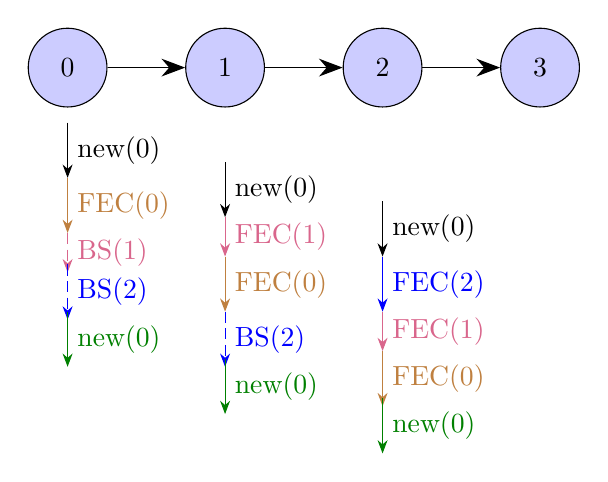
\begin{tikzpicture}
% Define circles with labels
\foreach \x [count=\i, evaluate=\i as \label using int(\i-1)] in {0,2,4,6} {
   \node[draw, circle, fill=blue!20, minimum size=1cm] (c\i) at (\x,0) {\label};
}
% Draw arrows between circles
\foreach \i in {1,2,3} {
   \pgfmathtruncatemacro{\next}{\i + 1}
   \draw[-{Stealth[length=3mm]}] (c\i) -- (c\next);
}
% First column lines
\draw ($(c1)+(0,-0.7)$) -- node[right, midway] {new(0)} ++(0,-0.7);
\draw [brown] ($(c1)+(0,-1.4)$) -- node[right, midway, brown] {FEC(0)} ++(0,-0.7);
\draw[purple!60, dash pattern=on 4pt off 2pt] ($(c1)+(0,-2.1)$) -- node[right, midway, purple!60] {BS(1)} ++(0,-0.5);
\draw[blue, dash pattern=on 4pt off 2pt] ($(c1)+(0,-2.5)$) -- node[right, midway, blue] {BS(2)} ++(0,-0.7);
\draw[green!50!black] ($(c1)+(0,-3.1)$) -- node[right, midway, green!50!black] {new(0)} ++(0,-0.7);
% Second column lines
\draw ($(c2)+(0,-1.2)$) -- node[right, midway] {new(0)} ++(0,-0.7);
\draw[purple!60] ($(c2)+(0,-1.9)$) -- node[right, midway, purple!60] {FEC(1)} ++(0,-0.5);
\draw [brown] ($(c2)+(0,-2.4)$) -- node[right, midway, brown] {FEC(0)} ++(0,-0.7);
\draw[blue, dash pattern=on 4pt off 2pt] ($(c2)+(0,-3.1)$) -- node[right, midway, blue] {BS(2)} ++(0,-0.7);
\draw[green!50!black] ($(c2)+(0,-3.7)$) -- node[right, midway, green!50!black] {new(0)} ++(0,-0.7);
% Third column lines
\draw ($(c3)+(0,-1.7)$) -- node[right, midway] {new(0)} ++(0,-0.7);
\draw[blue] ($(c3)+(0,-2.4)$) -- node[right, midway, blue] {FEC(2)} ++(0,-0.7);
\draw[purple!60] ($(c3)+(0,-3.1)$) -- node[right, midway, purple!60] {FEC(1)} ++(0,-0.5);
\draw[brown]($(c3)+(0,-3.6)$) -- node[right, midway, brown] {FEC(0)} ++(0,-0.7);
\draw[green!50!black] ($(c3)+(0,-4.2)$) -- node[right, midway, green!50!black] {new(0)} ++(0,-0.7);
\end{tikzpicture}} 
    \caption{\small
    % Blank-Spaces Emergence:
    The diagram illustrates how FEC periods at intermediate nodes create blank spaces at preceding nodes.
    Vertical lines represent each node transmission timeline, with packets labeled by type and generator node
    (The labels indicate the information added to the output DoF at each node).
    The colors indicate period lengths corresponding to each channel erasure rate. Dashed lines mark blank-space regions where packet transmissions may be ineffective.
    For example, FEC(0) represents a FEC period generated at node $0$ with length $ \lceil \hat{\epsilon}_0 \cdot \rm RTT_0 \rfloor$ and sent to node 1. Then, node $1$ first generates its own FEC period, FEC(1), before processing any DoF from FEC(0). This creates the time window BS(1) in node 0's timeline where any transmitted packets will not be immediately processed.
    Similarly, BS(2) propagates from node $2$'s FEC period. Since node $2$ cannot process packets during this time, node $1$ suspends transmission, which in turn allows node $0$ to pause as well. 
    }
    \label{fig:bl_sp}
    \vspace{-0.2cm}
\end{figure}

% \vspace{-0.9cm}
\noindent {\bf Network AC-RLNC (NET):}
At time slot $t$, node $n$ may receive feedback (line~\ref{line:inputs}) and 1) update its erasure rate estimation, 2) identify the forward bottleneck (line~\ref{line:estimation}), and 3) eliminate semi-decoded packets from the buffer (line~\ref{line:wmin}). The node then determines a transmission according to one of three states:
%
1) The a-priori FEC period (line~\ref{line:apriori}) is activated every $\rm RTT_n$ time slots (within the node's initial delay) and schedules FEC transmissions according to~\ref{itm:a-FEC}.
%
2) Once all a-priori FEC packets are sent, the blank-space period (BSP) is activated (lines~\ref{line:fec_check}-\ref{line:blank_end}). Its full operation is described in the next paragraph.
%
3) When no other period is active, the node operates in No-New No-FEC mode. It first checks if a FEC is needed using the end-of-window and the posterior FEC criteria (line~\ref{line:posterior}). If FEC is not required, the node transmits a new DoF - given that a new packet is available at the buffer. Otherwise, it pauses transmission (line~\ref{line:empty_tran}).

% Upon receiving feedback (line~\ref{line:inputs}), the node updates its erasure rate estimation, identifies the forward bottleneck node (line~\ref{line:estimation}), and eliminates semi-decoded packets (line~\ref{line:wmin}). 
% The elimination of semi-decoded packets effectively increments $w_{min}$ - the index of the oldest packet in the buffer.
% %
% The node then determines the appropriate output - a re-transmission, a pause, or a new packet. First, the node checks if the a-priori FEC period is activated (line~\ref{line:apriori}). This period is initiated every $\rm RTT_n$ time slots from the beginning of the node's operation (accounting for the node's initial delay).
% %
% Once the a-priori FEC period ends, the blank-space period is activated. Its full operation is described below (lines~\ref{line:fec_check}-\ref{line:blank_end}).
% %
% If neither period is active, the node implements the No-New No-FEC approach. It first checks for FEC requirements using either the end-of-window criterion or the posterior FEC requirement (line~\ref{line:posterior}). If FEC is not needed and a new packet is available in the buffer, the node incorporates this packet into the coded output packet (line~\ref{line:send_new}). Otherwise, if the buffer contains no new data and the node suspends transmission (line~\ref{line:empty_tran}).
%
% Note, only incoming packet containing valuable DoF is added to the node's buffer and considered a new packet in this node (i.e., re-transmissions that are not needed are discarded).

\setlength{\textfloatsep}{1pt}
\begin{algorithm}
\caption{Network AC-RLNC (NET)}
\label{alg:full_alg}
\begin{footnotesize}
\begin{algorithmic}[1]
    
    \STATE \textbf{Optional Inputs:} 
    From Previous Node: Input packet $c^{n-1}_{t-\rm RTT_{n-1}}$ (or $p_t$ for the first encoding node$^{\ref{comm:NoCode}}$, i.e., a source who encodes using \eqref{eqn:dof}); 
    From Next Node: Aggregated feedback $AF^n_t = \{F^{i}_{t'} |{t' \leq t - \sum_{k=i}^{N-1}\rm RTT_{k}}, \space i \in \{n+1, \ldots, N-1\}\}$. \label{line:inputs}
    % F^{i}_{t-(i-n)\rm RTT
    
    \STATE \textbf{Optional Outputs:} To Previous Node: Output aggregated feedback $\{F^n_t,AF^n_t\}$; 
    \smallskip
    To Next Node: Output packet $c^{n}_t$. \label{line:outputs}
    
    % \vspace{-0.2cm}
    \STATE \textbf{Estimation Update:} According to the feedback, update $\{\hat{\epsilon}_i \}_{n\leq i \leq N-2}$ using \eqref{eqn:eps_hat}, and the ${BN_n}$ \eqref{eqn: BN_n}. \label{line:estimation}
    
    \STATE \textbf{Eliminate Packets:} Using the feedback, assess and eliminate "semi-decoded" (\ref{term:semi_dec}) packets from the buffer. Update $w_{min}$ to the oldest packet.%accordingly. 
    \label{line:wmin}

    \colorbox{gray!10}{\parbox{\dimexpr\linewidth-2\fboxsep\relax}{%
    \STATE \textbf{A-Priori FEC period -~\ref{itm:a-FEC}.} \label{line:apriori}
    }}
    
    \smallskip
    \colorbox{blue!10}{\parbox{\dimexpr\linewidth-2\fboxsep\relax}{%
        \textbf{BLANK SPACE:} \label{line:blank_start}
        \IF{A-Priori FEC period is complete} \label{line:fec_check}
            \STATE Determine BS Basic Duration \ref{itm:BS-Period}:
            \smallskip
            \\$BS \gets \alpha \sum_{i=n+1}^{BN_n}{ \rm RTT_i \cdot\hat{\epsilon}_i}$ \label{line:bs_num}
            \smallskip
            \IF{$BS > 0$}
                \IF{$\Delta_t^{BS} > 1-\hat{\epsilon}_{BN_n}$ (BS Criterion \ref{itm:BS-Criterion})} \label{line:bs_crit}
                    \STATE Terminate BS period \label{line:bs_termin}
                
                \ELSE
                    \STATE Do not transmit \label{line:bs_empty}
                    \STATE $BS \gets BS-1$
                    \RETURN
                \ENDIF
            \ENDIF
        \ENDIF
    }} \label{line:blank_end}
    
    \smallskip
    \colorbox{gray!10}{\parbox{\dimexpr\linewidth-2\fboxsep\relax}{%   
    \textbf{No-New No-FEC:}
    
    \IF{ $w_{max}-w_{min}>w$ (EOW -~\ref{itm:EOW}) or $\Delta_t \geq 0$ (Posterior FEC -~\ref{itm:p-FEC})} \label{line:posterior}
        \STATE Send a re-transmission
    \ELSIF{New packet available in Buffer} \label{line:buffer_check}
        \STATE Increment $w_{\text{max}}$ by $1$; Send new packet \label{line:send_new}
    \ELSE
        \STATE Do not transmit \label{line:empty_tran}
    \ENDIF }}
    \RETURN \label{line:final_return}
\end{algorithmic}
\end{footnotesize}
\end{algorithm}

\vspace{-0.3cm}
\noindent {\bf BS Period (BSP):}
During this period, the node suspends transmissions. Once initiated, the period's duration is set as decribed in~\ref{itm:BS-Period} (line~\ref{line:bs_num}). Each time slot, the node evaluates if early termination is needed by the \ac{bsp}-criterion detailed in~\ref{itm:BS-Criterion} (lines~\ref{line:bs_crit}-\ref{line:bs_termin}).

\begin{figure*}[htbp]
    \centering
    \begin{subfigure}[t]{0.258\textwidth}
        \includegraphics[width=\linewidth,height=4cm]{figure_for_paper/Channel_Usage_Rate_All_vs_eps.png}
        \caption{\footnotesize Channel Usage Rate - $U, U_n$}
        \label{fig:global_channel_use}
    \end{subfigure}
    \hspace{-0.45cm}
    \begin{subfigure}[t]{0.258\textwidth}
        \includegraphics[width=\linewidth,height=4cm]{figure_for_paper/Node_-1_Data_Rates_vs_eps.png}
        \caption{\footnotesize $R_{\rm del}$ and $\eta$}
        \label{fig:global_rate}
    \end{subfigure}
    \hspace{-0.45cm}
    \begin{subfigure}[t]{0.258\textwidth}
        \includegraphics[width=\linewidth,height=4cm]{figure_for_paper/Mean_Delay_All_vs_eps.png}
        \caption{\footnotesize Mean Delay [Slots] - $D^{\rm mean}$}
        \label{fig:global_mean_d}
    \end{subfigure}
    \hspace{-0.45cm}
    \begin{subfigure}[t]{0.258\textwidth}
        \includegraphics[width=\linewidth,height=4cm]{figure_for_paper/Max_Delay_All_vs_eps.png}
        \caption{\footnotesize Max Delay [Slots] - $D^{\rm max}$}
        \label{fig:global_max_d}
    \end{subfigure}
    
    \caption{\small System performance of 6-nodes network with respect to $\epsilon_2$ where $\epsilon_0=\epsilon_5=0.1$, $\epsilon_2=0.4$. 
    %When $\epsilon_2 > 0.4$ it is the global bottleneck.
    % The global bottleneck shifts when $\epsilon_2>0.4$
    }
    \label{fig:global_metrics}
    \vspace{-0.45cm}
\end{figure*}



\vspace{-0.05cm}

\begin{enumerate}[wide, labelwidth=0.3cm, labelindent=1pt, label=\textcolor{blue}{M-BS-\arabic*}, itemsep=1em]

\item \label{itm:BS-Period}
\textit{\underline{\ac{bsp} Duration}:} %
The \ac{bsp} duration is determined based on the a priori FEC periods of subsequent nodes in the network and considering the following:
%
1) While nodes transmit FEC relative to their newly transmitted DoFs ($c_{t}^{\text{new}}$,~\ref{itm:a-FEC}), this information isn't directly available through feedback links. However, estimation of the subsequent links' erasure rates is available by backward feedback aggregation $AF^n_t$ (lines~\ref{line:inputs}-\ref{line:outputs}).
%and similarly to \eqref{eqn:eps_hat} due to propagation delay.
%%%%%%%%% Extra explanation for the long version: %%%%%%%%%
% That is, at time $t$, node $n$ receives all ACKs and NACKs from the next nodes. Specifically, each node sends back both its local feedback $F^n_t$ and aggregated feedback $AF^n_t$ to the previous node, so the aggregated feedback $AF^n_t$ contains acknowledgments $F_{t'}^i$ from nodes $n+1$ to $N-1$ at times $t'$ not exceeding $t - \sum_{k=i}^{N-1}\rm RTT_{k}$. $\hat{\epsilon}_n$ computed as the mean of all relevant channel acknowledgments per \eqref{eqn:eps_hat}.
That is, the destination node sends back an ACK/NACK message to node N-1, which in turn sends back two things: its own feedback message, along with the feedback message it received from the destination. Then node N-1 sends both messages to node N-2, which adds its own feedback and passes all three messages back. This process continues backwards through the chain, where each node sends back its own feedback message $F^n_t$ and the collection of messages it received from the next node denoted by $AF^n_t$. Specifically, $AF^n_t$ contains acknowledgments $F_{t'}^i$ from nodes $n+1$ to $N-1$ at times $t'$ not exceeding $t - \sum_{k=i}^{N-1}\rm RTT_{k}$. The erasure rate of each preceding channel $\hat{\epsilon}_n$ is then computed as the mean of all its corresponding acknowledgments in $AF^n_t$ by \eqref{eqn:eps_hat}.
%%%%%%%%%%%%%%%%%%%%%%%%%%%%%%%%%%%%%%%%%%%%%%%%%%%%%%
%
2) The forward-channels bottleneck link, which requires the highest FEC transmission, constrains the local theoretical capacity and contributes the most \ac{bsp} slots. Any packet at this link should be forwarded immediately to maintain high transmission rates, regardless of subsequent channel conditions.
%
Therefore, the \ac{bsp} duration considers two factors: the basic window of new DoFs for each $i$th hop - $\rm RTT_i$, and the estimated erasure rates up to the forward bottleneck, resulting, for node $n$ at time $t$ as
%
\begin{equation}
 \textstyle   BS_n(t) = \begin{cases}
\textstyle         \alpha \sum_{i=n+1}^{BN_n} \rm RTT_i \cdot\hat{\epsilon}_i & \hspace{-0.2cm}\text{if } n<BN_n, \text{ using Eq.\hspace{-0.1cm}~\eqref{eqn: BN_n}} \\
\textstyle        0 & \hspace{-0.2cm}\text{if } n=BN_n
    \end{cases}
    \label{eqn:BS_num}
\end{equation}
%
where $\alpha$ is a tuneable parameter used to relax the evaluation error.
Note that if channel $e_n$ is the forward bottleneck itself, we set $BS_n(t)=0$, eliminating any transmission suspension.

\vspace{-0.2cm}
\item \label{itm:BS-Criterion}
\textit{\underline{BS Termination Criterion}:}
Transmission suspension can be considered a packet erasure, allowing us to analyze this through the DoF rate framework given in \eqref{eqn:delta_new}. We want to identify the critical point where further suspension would degrade the data rate performance.
%
To model this, we set $md_{t}^{\text{nack}}=1$, representing guaranteed packet erasure, with the remaining \ac{bsp} window available for re-transmissions compensation. Since only FEC are considered, $c_{t}^{\text{new}}=0$, and with uncertain delivery, $ad_{t}^{\text{ack}}=0$. 
Finally, $c_{t}^{\text{same}}=BS_n(t)$, representing the number of re-transmissions with unknown delivery status.
% Importance term
While a node's transmission rate is constrained by its forward channels bottleneck, channels with similar erasure rates can have significant impact as well. To quantify this, we consider both the erasure rate differential between the current channel and its bottleneck, and their distance in hops, denoted by $h = BN_n - n$.
%
This sets the \ac{bsp}-DoF rate by
\begin{equation*}
\textstyle    \Delta_t^{BS} = \left[ \left( 1-\hat{\epsilon}_n \right) BS(t)+h\log(\hat{\epsilon}_{BN_n}-\hat{\epsilon}_n) \right] ^{-1}.
\end{equation*}
\off{recalling that $\epsilon_n$ represents the erasure probability at node $n$.}
%
To ensure suspending transmission doesn't reduce the rate below the capacity, we compare the \ac{bsp} DoF rate to the forward bottleneck rate. 
Thus, the \ac{bsp} is terminated when,
\begin{equation}
\textstyle    \Delta_t^{BS} > 1-\hat{\epsilon}_{BN_n}.
    \label{BS_crit}
\end{equation}
%
This criterion identifies the critical point where the remaining transmission slots, $BS_n(t)$, are the slots needed to compensate for the "missing" DoF. Any further pause would likely result in a rate reduction.

\end{enumerate}

% \vspace{-0.1cm}
% \section{Evaluation Results}
% \label{sec:EvalRes}
% % Intro
% In this section, we present simulation results of the \ac{bs-acrlnc} protocol\footnote{The code is available at \url{https://github.com/Adinawx/MH_NC}}.
% % Simulation setup
% We evaluate a 6-node network with BEC channels, where $\epsilon_0=\epsilon_5=0.1$, $\epsilon_1=0.4$, $\epsilon_3=0.3$, and middle link $\epsilon_2$ varies from $0.2$ to $0.6$. Information packets arrive at the source according to a Bernoulli process with rate $1-\epsilon_{BN} - 0.1$. We set $\rm RTT_n=20$ for each node $n$, yielding a global $\rm RTT$ of $100$ slots over a time horizon of $T=5000$ slots.
% % Algorithms
% We compare four algorithms: 
% 1) The proposed \ac{bs-acrlnc} ('BS'); 
% 2) 'NET-FEC', a \ac{bs-acrlnc} version which performs \ac{net-acrlnc} without idle periods - the BS period is eliminated and No-New No-FEC pauses are replaced with FEC transmissions;
% % 2) 'NET-FEC', performs \ac{net-acrlnc} without idle periods
% 3) 'Baseline' using MP-MH AC-RLNC, implementing AC-RLNC only at the source with basic re-encoding at intermediate nodes (see Sec.~\ref{subsec:MPMH}); 
% and 4) common non-coded selective repeat ARQ ('SR-ARQ') \cite{weldon1982improved}.
% % Graphs
% In Fig.\ref{fig:global_channel_use}, we present the channel usage rate for each node and for the end-to-end network~\eqref{eqn:channel_use}. 
% The channel usage generally decreases as the global bottleneck becomes more severe, %This illustrates how the \ac{bs-acrlnc} algorithm enables individual nodes to leverage the network bottleneck limitation. 
% with the notable exception of the middle node (in red). This node is connected to the varying channel and its activity level increases with its erasure rate, reaching maximum utilization (rate of 1) when it becomes the bottleneck, for $\epsilon_2 \geq 0.5$.
% In the end-to-end graph, we observe a $20\%$ reduction for a bottleneck of $0.4$, with this effect becoming more pronounced as the bottleneck shifts across the network. 
% %
% Notably, we maintain a delivery rate nearly identical to the baseline measurements as seen in Fig.~\ref{fig:global_rate}. For all algorithms except \ac{bs-acrlnc}, the goodput and delivery rate differ by less than $1\%$, thus represented by a single line. The \ac{bs-acrlnc} goodput is presented separately as it achieves significantly higher performance.
% %
% The in-order delivery delay metrics of all the AC-RLNC solutions are upper-bounded in mean and max metrics by $400$ and $750$ time slots, respectively. The overall difference between the compared solutions remains within approximately two global $\rm RTT$. As demonstrated in \cite{dias2023sliding}, these delays meet the standard requirements for URLLC, and are one-order better than rateless RLNC \cite{bonello2011myths}, and two-orders better than non-coded solutions with UDP and selective repeat ARQ \cite{weldon1982improved}, which are typically used in TCP layers (discussed also in \cite{dias2023sliding,cohen2021bringing,cohen2020adaptiveMH}).  

% \noindent\textit{\bf Future Work and Discussion:}
% Based on these promising results, we propose two key directions for further investigation. Investigating varying RTTs between nodes could improve our approach by allowing nodes with faster connections to pause while waiting for slower channels. Extending to multipath-multihop scenarios would also enable smarter transmission scheduling through idle nodes, enhancing network efficiency. For single-source multicast scenario, we present results in \cite{BS-ACRLNC}. 



\vspace{-0.1cm}
\section{Evaluation Results}
\label{sec:EvalRes}
% Intro
In this section, we present simulation results demonstrating the effectiveness of the \ac{bs-acrlnc} protocol \footnote{The simulations code is available at \url{https://github.com/Adinawx/MH_NC}}.
% Simulation Configuration
We evaluate a 6-node network with BEC channels, where $\epsilon_0=\epsilon_5=0.1$, $\epsilon_1=0.4$, $\epsilon_3=0.3$, and middle link $\epsilon_2$ varies from $0.2$ to $0.6$ across simulations. The global bottleneck remains $\epsilon_{BN}=\epsilon_1=0.4$ until $\epsilon_2$ exceeds $0.4$ and becomes the global bottleneck itself.
Considering the capacity limit, information packets arrive at the source according to a Bernoulli process with a rate slightly lower than the global bottleneck, $1-\epsilon_{BN} - 0.1$. We set $\rm RTT_n=20$ for each node $n$, yielding a global $\rm RTT$ of $100$ slots over a time horizon of $T=5000$ slots.
%
We compare four algorithms: 
1) The proposed \ac{bs-acrlnc} ('BS').
%
2) 'NET-FEC', a \ac{bs-acrlnc} version which performs \ac{net-acrlnc} without idle periods - the BS period is eliminated and No-New No-FEC pauses are replaced with FEC transmissions - This allows us to evaluate the effect of the idle periods distinctively.
%
3) 'Baseline' using MP-MH AC-RLNC, implementing AC-RLNC only at the source with basic re-encoding at intermediate nodes (see Sec.~\ref{subsec:MPMH}); 
%
and 4) common non-coded selective repeat ARQ ('SR-ARQ') \cite{weldon1982improved}.
%
% Overall View
In Fig.~\ref{fig:global_metrics}, we present the channel usage savings compared to the rate and delay metrics. 
% Channel Usage
In Fig.\ref{fig:global_channel_use}, we present the channel usage rate for each node separately and for the end-to-end network~\eqref{eqn:channel_use}. 
While NET-FEC, Baseline, and SR-ARQ operate at maximum channels utilization (rate of 1), \ac{bs-acrlnc} achieves significant reductions
% Individual channels
Examining each node, channel usage typically decreases as the global bottleneck becomes more severe and shifts position at $\epsilon_2 \geq 0.4$, demonstrating how \ac{bs-acrlnc} nodes adapt to network bottleneck constraints. Node $2$, however, shows distinct behavior: its activity increases with its erasure rate, reaching maximum utilization when it becomes the bottleneck.
% End-to-end
The end-to-end performance (blue stars) reveals that overall channel usage decreases with increasing erasure rate, highlighting \ac{bs-acrlnc}'s network-level benefits. We observe a $20\%$ reduction in channel usage when $\epsilon_1=0.4$ is the bottleneck, with even greater efficiency gains as the bottleneck shifts across the network.
% Data Rates
In Fig.~\ref{fig:global_rate}, we present goodput and delivery rates. The metrics are nearly identical (within $0.01$) for all algorithms except \ac{bs-acrlnc}, and are thus given by a single line. \ac{bs-acrlnc} shows significantly higher goodput, indicated by the dashed line with upward triangles, due to its transmission pauses.
%
Notably, \ac{bs-acrlnc} reduces channel usage, while maintaining a delivery rate comparable to the coding algorithms and outperforms the SR-ARQ. This demonstrates the algorithm does not compromise its delivery performance for reducing channel usage.
%
% Delay
The in-order delivery delay metrics of all the AC-RLNC solutions are upper-bounded in mean and max metrics by $400$ and $750$ time slots, respectively. The overall difference between the compared solutions remains within approximately two global $\rm RTT$. As demonstrated in \cite{dias2023sliding}, these delays meet the standard requirements for URLLC, and are one-order better than rateless RLNC \cite{bonello2011myths}, and two-orders better than non-coded solutions with UDP and selective repeat ARQ \cite{weldon1982improved}, which are typically used in TCP layers (discussed also in \cite{dias2023sliding,cohen2021bringing,cohen2020adaptiveMH}).  
%
% Multi Cast Results:
In Fig~\ref{fig:multicast} we present a single-source multicast scenario where all intermediate nodes function as destinations, decoding the information packets. Note that this decoding does not affect the algorithm's operation, which continues to function in its original semi-decoding manner.
% AC Delay
The results for both BS and NET-FEC demonstrate how delay varies with respect to the bottleneck channel position. The first node (Fig~\ref{fig:mc_1}) experiences a minimal delay, consistent with the expected AC-RLNC algorithm performance. At the second node (Fig~\ref{fig:mc_2}), we observe two distinct behaviors: high delay when $\epsilon\leq 0.4$ due to transmission over the bottleneck channel, and low delay when $\epsilon>0.4$ as the bottleneck shifts further downstream in the network. The remaining nodes  (Fig~\ref{fig:mc_3}-Fig~\ref{fig:mc_5}) exhibit higher delays as they are all affected by the bottleneck channel.
% AC Rates
The goodput and delivery rate results align with our multi-hop findings (Fig~\ref{fig:bl_sp}). These metrics remain consistent across nodes since all algorithms consider the end-to-end network conditions rather than local information. While the delivery rate shows a slight decrease with distance from the source due to cumulative erasures, this could be improved through better erasure rate estimation.
% Baseline
The baseline solution demonstrates stable rate and delay performance due to its global approach, though at the cost of higher channel usage as shown in Fig.~\ref{fig:global_channel_use}. 
% SR ARQ
While SR-ARQ achieves competitive performance at the first node, its performance degrades significantly at subsequent nodes. Unlike the coding solutions, which consider the entire 6-node network, SR-ARQ operates locally at each node. This leads to high delivery rates at the initial nodes but declining performance when reaching bottleneck nodes. Since the multicast scenario requires uniform delivery rates across all nodes, this initial advantage becomes irrelevant.
% Channel Usage
Each channel usage rate is seen in (Fig~\ref{fig:bl_sp}).
% Conclusion:
These results demonstrate that \ac{bs-acrlnc} achieves significant improvements in channel usage and goodput while maintaining baseline delivery rate and low delay performance, validating the effectiveness of the proposed approach.

\noindent\textit{\bf Future Work and Discussion:}
Based on these promising results, we propose two key directions for further investigation. Investigating varying RTTs between nodes could improve our approach by allowing nodes with faster connections to pause while waiting for slower channels. Extending to multipath-multihop scenarios would also enable smarter transmission scheduling through idle nodes, enhancing network efficiency. %For single-source multicast scenario, we present results in \cite{BS-ACRLNC}. 


\begin{figure*}[htbp]
    \vspace{-1.8cm}

   \centering
   \begin{subfigure}[b]{0.6\textwidth}
       \includegraphics[width=\textwidth]{figures_for_arxiv/multi-cast/Node_1_Combined_Metrics_vs_eps.png}
       \caption{\small Node 1. The capacity for SR-ARQ is 0.9.}
       \label{fig:mc_1}
   \end{subfigure}
   \begin{subfigure}[b]{0.6\textwidth}
       \includegraphics[width=\textwidth]{figures_for_arxiv/multi-cast/Node_2_Combined_Metrics_vs_eps.png}
       \caption{\small Node 2. The capacity for SR-ARQ is 0.6.}
       \label{fig:mc_2}
   \end{subfigure}
   \begin{subfigure}[b]{0.6\textwidth}
       \includegraphics[width=\textwidth]{figures_for_arxiv/multi-cast/Node_3_Combined_Metrics_vs_eps.png}
       \caption{\small Node 3. The capacity for SR-ARQ is $\epsilon_2$.}
       \label{fig:mc_3}
   \end{subfigure}
   \\
   \begin{subfigure}[b]{0.6\textwidth}
       \includegraphics[width=\textwidth]{figures_for_arxiv/multi-cast/Node_4_Combined_Metrics_vs_eps.png}
       \caption{\small Node 4. The capacity for SR-ARQ is $\epsilon_2$.}
       \label{fig:mc_4}
   \end{subfigure}
   \begin{subfigure}[b]{0.6\textwidth}
       \includegraphics[width=\textwidth]{figures_for_arxiv/multi-cast/Node_5_Combined_Metrics_vs_eps.png}
       \caption{\small Node 5. The capacity for SR-ARQ is $\epsilon_2$.}
       \label{fig:mc_5}
   \end{subfigure}
   \caption{\small Analysis of multi-cast Scenario when all nodes function as destinations.}

   \label{fig:multicast}
\end{figure*}


\begin{comment}


\begin{figure*}[htbp]
    \centering

    \begin{subfigure}[t]{0.258\textwidth}
        \includegraphics[width=\linewidth,height=4cm]{figures_for_arxiv/multi-cast/Node_1_Data_Rates_vs_eps.png}
        \caption{\footnotesize Data Rates}
        \label{fig:global_del_rate}
    \end{subfigure}
    % \hspace{-0.45cm}
    % \hspace{-0.45cm}
    \begin{subfigure}[t]{0.258\textwidth}
        \includegraphics[width=\linewidth,height=4cm]{figures_for_arxiv/multi-cast/Mean Real Delay_1_vs_eps.png}
        \caption{\footnotesize Mean Delay [Slots] - $D^{\rm mean}$}
        \label{fig:global_goodput}
    \end{subfigure}
    % \hspace{-0.45cm}
    \begin{subfigure}[t]{0.258\textwidth}
        \includegraphics[width=\linewidth,height=4cm]{figures_for_arxiv/multi-cast/Max_Real_Delay_1_vs_eps.png}
        \caption{\footnotesize Max Delay [Slots] - $D^{\rm max}$}
        \label{fig:all_channels}
    \end{subfigure}
    
    \caption{\small node 1 is the destination}
    \label{fig:global_metrics}
    \vspace{-0.45cm}
\end{figure*}

\begin{figure*}[htbp]
    \centering
    \begin{subfigure}[t]{0.258\textwidth}
        \includegraphics[width=\linewidth,height=4cm]{figures_for_arxiv/multi-cast/Node_2_Data_Rates_vs_eps.png}
        \caption{\footnotesize Data Rates}
        \label{fig:global_del_rate_2}
    \end{subfigure}
    % \hspace{-0.45cm}
    % \hspace{-0.45cm}
    \begin{subfigure}[t]{0.258\textwidth}
        \includegraphics[width=\linewidth,height=4cm]{figures_for_arxiv/multi-cast/Mean_Real_Delay_2_vs_eps.png}
        \caption{\footnotesize Mean Delay [Slots] - $D^{\rm mean}$}
        \label{fig:global_goodput_2}
    \end{subfigure}
    % \hspace{-0.45cm}
    \begin{subfigure}[t]{0.258\textwidth}
        \includegraphics[width=\linewidth,height=4cm]{figures_for_arxiv/multi-cast/Max_Real_Delay_2_vs_eps.png}
        \caption{\footnotesize Max Delay [Slots] - $D^{\rm max}$}
        \label{fig:all_channels_2}
    \end{subfigure}
    
    \caption{\small node 2 is the destination}
    \label{fig:global_metrics_2}
    \vspace{-0.45cm}
\end{figure*}

\begin{figure*}[htbp]
    \centering
    \begin{subfigure}[t]{0.258\textwidth}
        \includegraphics[width=\linewidth,height=4cm]{figures_for_arxiv/multi-cast/Node_3_Data_Rates_vs_eps.png}
        \caption{\footnotesize Data Rates}
        \label{fig:global_del_rate_3}
    \end{subfigure}
    % \hspace{-0.45cm}
    % \hspace{-0.45cm}
    \begin{subfigure}[t]{0.258\textwidth}
        \includegraphics[width=\linewidth,height=4cm]{figures_for_arxiv/multi-cast/Mean Real Delay_3_vs_eps.png}
        \caption{\footnotesize Mean Delay [Slots] - $D^{\rm mean}$}
        \label{fig:global_goodput_3}
    \end{subfigure}
    % \hspace{-0.45cm}
    \begin{subfigure}[t]{0.258\textwidth}
        \includegraphics[width=\linewidth,height=4cm]{figures_for_arxiv/multi-cast/Max_Real_Delay_3_vs_eps.png}
        \caption{\footnotesize Max Delay [Slots] - $D^{\rm max}$}
        \label{fig:all_channels_3}
    \end{subfigure}
    
    \caption{\small node 3 is the destination}
    \label{fig:global_metrics_3}
    \vspace{-0.45cm}
\end{figure*}

\begin{figure*}[htbp]
    \centering
    \begin{subfigure}[t]{0.258\textwidth}
        \includegraphics[width=\linewidth,height=4cm]{figures_for_arxiv/multi-cast/Node_4_Data_Rates_vs_eps.png}
        \caption{\footnotesize Data Rates}
        \label{fig:global_del_rate_4}
    \end{subfigure}
    % \hspace{-0.45cm}
    % \hspace{-0.45cm}
    \begin{subfigure}[t]{0.258\textwidth}
        \includegraphics[width=\linewidth,height=4cm]{figures_for_arxiv/multi-cast/Mean Real Delay_4_vs_eps.png}
        \caption{\footnotesize Mean Delay [Slots] - $D^{\rm mean}$}
        \label{fig:global_goodput_4}
    \end{subfigure}
    % \hspace{-0.45cm}
    \begin{subfigure}[t]{0.258\textwidth}
        \includegraphics[width=\linewidth,height=4cm]{figures_for_arxiv/multi-cast/Max_Real_Delay_4_vs_eps.png}
        \caption{\footnotesize Max Delay [Slots] - $D^{\rm max}$}
        \label{fig:all_channels_4}
    \end{subfigure}
    
    \caption{\small node 4 is the destination}
    \label{fig:global_metrics_4}
    \vspace{-0.45cm}
\end{figure*}

\begin{figure*}[htbp]
    \centering
    \begin{subfigure}[t]{0.258\textwidth}
        \includegraphics[width=\linewidth,height=4cm]{figures_for_arxiv/multi-cast/Node_5_Data_Rates_vs_eps.png}
        \caption{\footnotesize Data Rates}
        \label{fig:global_del_rate_5}
    \end{subfigure}
    % \hspace{-0.45cm}
    % \hspace{-0.45cm}
    \begin{subfigure}[t]{0.258\textwidth}
        \includegraphics[width=\linewidth,height=4cm]{figures_for_arxiv/multi-cast/Mean Real Delay_5_vs_eps.png}
        \caption{\footnotesize Mean Delay [Slots] - $D^{\rm mean}$}
        \label{fig:global_goodput_5}
    \end{subfigure}
    % \hspace{-0.45cm}
    \begin{subfigure}[t]{0.258\textwidth}
        \includegraphics[width=\linewidth,height=4cm]{figures_for_arxiv/multi-cast/Max_Real_Delay_5_vs_eps.png}
        \caption{\footnotesize Max Delay [Slots] - $D^{\rm max}$}
        \label{fig:all_channels_5}
    \end{subfigure}
    
    \caption{\small node 5 is the destination}
    \label{fig:global_metrics_5}
    \vspace{-0.45cm}
\end{figure*}

\end{comment}

%%%%%%%%%%%%%%%%%%%%%%%%%%%%%
%%%%%%%
% \subsection{Templates}


% The paper (A4 or letter size, double-column format, not exceeding 5 pages plus an optional 6th page only containing references) should be formatted as shown in this sample \LaTeX{} file
% \cite{Laport:LaTeX, GMS:LaTeXComp, oetiker_latex, typesetmoser}.


% The use of Microsoft Word or other text processing systems instead of \LaTeX{} is strongly
% discouraged. Users of such systems should attempt to duplicate the
% style of this example, in particular the sizes and type of font, as
% closely as possible.




% \subsection{Formatting}


% The style of references, equations, figures, tables, etc. should be
% the same as for the \emph{IEEE Transactions on Information
%   Theory}. 
  
%   The source file of this template paper contains many more
% instructions on how to format your paper. For example, example code for
% different numbers of authors, for figures and tables, and references
% can be found (they are commented out).




%%%%%%
%% An example of a floating figure using the graphicx package.
%% Note that \label must occur AFTER (or within) \caption.
%% For figures, \caption should occur after the \includegraphics.
%%
% \begin{figure}[htbp]
%   \centering
%   \includegraphics[width=0.3\textwidth]{myfigure}
%   % where an .eps filename suffix will be assumed under latex,
%   % and a .pdf suffix will be assumed for pdflatex
%   \caption{Simulation results.}
%   \label{fig:sim}
% \end{figure}
%%%%%%


%%%%%%
%% An example of a double column floating figure using two subfigures.
%% (The subfigure.sty package must be loaded for this to work.)  The
%% subfigure \label commands are set within each subfigure command,
%% the \label for the overall figure must come after \caption.  
%% \hfil must be used as a separator to get equal spacing
%%
% \begin{figure*}[htbp]
%   \centerline{\subfigure[Case I]{\includegraphics[width=2.5in]{subfigcase1}
%       % where an .eps filename suffix will be assumed under latex,
%       % and a .pdf suffix will be assumed for pdflatex
%       \label{fig:first_case}}
%     \hfil
%     \subfigure[Case II]{\includegraphics[width=2.5in]{subfigcase2}
%       % where an .eps filename suffix will be assumed under latex,
%       % and a .pdf suffix will be assumed for pdflatex
%       \label{fig:second_case}}}
%   \caption{Simulation results.}
%   \label{fig:sim}
% \end{figure*}
%%%%%%


%%%%%%
%% An example of a floating table. 
%% Note that, for IEEE style tables, the \caption command should come
%% BEFORE the table. Table text will default to \footnotesize as IEEE
%% normally uses this smaller font for tables. The \label must come
%% after \caption as always.
%%
% \begin{table}[htbp]
%   % increase table row spacing, adjust to taste
%   \renewcommand{\arraystretch}{1.3}
%   \caption{An Example of a Table}
%   \label{tab:table_example}
%   \centering
%   % Some packages, such as MDW tools, offer better commands for making tables
%   % than the plain LaTeX2e tabular which is used here.
%   \begin{tabular}{|c||c|}
%     \hline
%     One & Two\\
%     \hline
%     Three & Four\\
%     \hline
%   \end{tabular}
% \end{table}
%%%%%%


% For instructions on how to typeset math, in particular for equation
% arrays with broken equations, we refer to \cite{typesetmoser}.


% Final papers should have no page numbers and no headers or footers (both will be added during the production of the proceedings).
% The top and bottom margins should be at least 0.5 inches to leave room for page numbers.
% All fonts should be embedded in the pdf file.




%%%%%%
%% Appendix:
%% If needed a single appendix is created by
%%
%\appendix
%%
%% If several appendices are needed, then the command
%%
% \appendices
%%
%% in combination with further \section commands can be used.
%%%%%%


%\section*{Acknowledgment}




%%%%%%
%% To balance the columns at the last page of the paper use this
%% command:
%%
%\enlargethispage{-1.2cm} 
%%
%% If the balancing should occur in the middle of the references, use
%% the following trigger:
%%
%\IEEEtriggeratref{7}
%%
%% which triggers a \newpage (i.e., new column) just before the given
%% reference number. Note that you need to adapt this if you modify
%% the paper.  The "triggered" command can be changed if desired:
%%
%\IEEEtriggercmd{\enlargethispage{-20cm}}
%%
%%%%%%




%%%%%%
%% References:
%% We recommend the usage of BibTeX:
%%
%\bibliographystyle{IEEEtran}
%\bibliography{definitions,bibliofile}
%%
%% where we here have assumed the existence of the files
%% definitions.bib and bibliofile.bib.
%% BibTeX documentation can be obtained at:
%% http://www.ctan.org/tex-archive/biblio/bibtex/contrib/doc/
%%%%%%


%\newpage
%%%%%%%%%%%%%%%%%%%%%%%%%%%%%%%%%%%%%%%%%%%%%%%%%%%%%
\bibliographystyle{IEEEtran}
\bibliography{main}
%%%%%%%%%%%%%%%%%%%%%%%%%%%%%%%%%%%%%%%%%%%%%%%%%%%%%


\end{document}




%%%%%%
%% Some comments about useful packages
%% (extract from bare_conf.tex by Michael Shell)
%%


% *** MISC UTILITY PACKAGES ***
%
%\usepackage{ifpdf}
% Heiko Oberdiek's ifpdf.sty is very useful if you need conditional
% compilation based on whether the output is pdf or dvi.
% usage:
% \ifpdf
%   % pdf code
% \else
%   % dvi code
% \fi
% The latest version of ifpdf.sty can be obtained from:
% http://www.ctan.org/pkg/ifpdf
% Also, note that IEEEtran.cls V1.7 and later provides a builtin
% \ifCLASSINFOpdf conditional that works the same way.
% When switching from latex to pdflatex and vice-versa, the compiler may
% have to be run twice to clear warning/error messages.




% *** CITATION PACKAGES ***
%
%\usepackage{cite}
% cite.sty was written by Donald Arseneau
% V1.6 and later of IEEEtran pre-defines the format of the cite.sty package
% \cite{} output to follow that of the IEEE. Loading the cite package will
% result in citation numbers being automatically sorted and properly
% "compressed/ranged". e.g., [1], [9], [2], [7], [5], [6] without using
% cite.sty will become [1], [2], [5]--[7], [9] using cite.sty. cite.sty's
% \cite will automatically add leading space, if needed. Use cite.sty's
% noadjust option (cite.sty V3.8 and later) if you want to turn this off
% such as if a citation ever needs to be enclosed in parenthesis.
% cite.sty is already installed on most LaTeX systems. Be sure and use
% version 5.0 (2009-03-20) and later if using hyperref.sty.
% The latest version can be obtained at:
% http://www.ctan.org/pkg/cite
% The documentation is contained in the cite.sty file itself.




% *** GRAPHICS RELATED PACKAGES ***
%
\ifCLASSINFOpdf
  % \usepackage[pdftex]{graphicx}
  % declare the path(s) where your graphic files are
  % \graphicspath{{../pdf/}{../jpeg/}}
  % and their extensions so you won't have to specify these with
  % every instance of \includegraphics
  % \DeclareGraphicsExtensions{.pdf,.jpeg,.png}
\else
  % or other class option (dvipsone, dvipdf, if not using dvips). graphicx
  % will default to the driver specified in the system graphics.cfg if no
  % driver is specified.
  % \usepackage[dvips]{graphicx}
  % declare the path(s) where your graphic files are
  % \graphicspath{{../eps/}}
  % and their extensions so you won't have to specify these with
  % every instance of \includegraphics
  % \DeclareGraphicsExtensions{.eps}
\fi
% graphicx was written by David Carlisle and Sebastian Rahtz. It is
% required if you want graphics, photos, etc. graphicx.sty is already
% installed on most LaTeX systems. The latest version and documentation
% can be obtained at: 
% http://www.ctan.org/pkg/graphicx
% Another good source of documentation is "Using Imported Graphics in
% LaTeX2e" by Keith Reckdahl which can be found at:
% http://www.ctan.org/pkg/epslatex
%
% latex, and pdflatex in dvi mode, support graphics in encapsulated
% postscript (.eps) format. pdflatex in pdf mode supports graphics
% in .pdf, .jpeg, .png and .mps (metapost) formats. Users should ensure
% that all non-photo figures use a vector format (.eps, .pdf, .mps) and
% not a bitmapped formats (.jpeg, .png). The IEEE frowns on bitmapped formats
% which can result in "jaggedy"/blurry rendering of lines and letters as
% well as large increases in file sizes.
%
% You can find documentation about the pdfTeX application at:
% http://www.tug.org/applications/pdftex




% *** MATH PACKAGES ***
%
%\usepackage{amsmath}
% A popular package from the American Mathematical Society that provides
% many useful and powerful commands for dealing with mathematics.
%
% Note that the amsmath package sets \interdisplaylinepenalty to 10000
% thus preventing page breaks from occurring within multiline equations. Use:
%\interdisplaylinepenalty=2500
% after loading amsmath to restore such page breaks as IEEEtran.cls normally
% does. amsmath.sty is already installed on most LaTeX systems. The latest
% version and documentation can be obtained at:
% http://www.ctan.org/pkg/amsmath




% *** SPECIALIZED LIST PACKAGES ***
%
%\usepackage{algorithmic}
% algorithmic.sty was written by Peter Williams and Rogerio Brito.
% This package provides an algorithmic environment for describing algorithms.
% You can use the algorithmic environment in-text or within a figure
% environment to provide for a floating algorithm. Do NOT use the algorithm
% floating environment provided by algorithm.sty (by the same authors) or
% algorithm2e.sty (by Christophe Fiorio) as the IEEE does not use dedicated
% algorithm float types and packages that provide these will not provide
% correct IEEE style captions. The latest version and documentation of
% algorithmic.sty can be obtained at:
% http://www.ctan.org/pkg/algorithms
% Also of interest may be the (relatively newer and more customizable)
% algorithmicx.sty package by Szasz Janos:
% http://www.ctan.org/pkg/algorithmicx




% *** ALIGNMENT PACKAGES ***
%
%\usepackage{array}
% Frank Mittelbach's and David Carlisle's array.sty patches and improves
% the standard LaTeX2e array and tabular environments to provide better
% appearance and additional user controls. As the default LaTeX2e table
% generation code is lacking to the point of almost being broken with
% respect to the quality of the end results, all users are strongly
% advised to use an enhanced (at the very least that provided by array.sty)
% set of table tools. array.sty is already installed on most systems. The
% latest version and documentation can be obtained at:
% http://www.ctan.org/pkg/array


% IEEEtran contains the IEEEeqnarray family of commands that can be used to
% generate multiline equations as well as matrices, tables, etc., of high
% quality.




% *** SUBFIGURE PACKAGES ***
%\ifCLASSOPTIONcompsoc
%  \usepackage[caption=false,font=normalsize,labelfont=sf,textfont=sf]{subfig}
%\else
%  \usepackage[caption=false,font=footnotesize]{subfig}
%\fi
% subfig.sty, written by Steven Douglas Cochran, is the modern replacement
% for subfigure.sty, the latter of which is no longer maintained and is
% incompatible with some LaTeX packages including fixltx2e. However,
% subfig.sty requires and automatically loads Axel Sommerfeldt's caption.sty
% which will override IEEEtran.cls' handling of captions and this will result
% in non-IEEE style figure/table captions. To prevent this problem, be sure
% and invoke subfig.sty's "caption=false" package option (available since
% subfig.sty version 1.3, 2005/06/28) as this is will preserve IEEEtran.cls
% handling of captions.
% Note that the Computer Society format requires a larger sans serif font
% than the serif footnote size font used in traditional IEEE formatting
% and thus the need to invoke different subfig.sty package options depending
% on whether compsoc mode has been enabled.
%
% The latest version and documentation of subfig.sty can be obtained at:
% http://www.ctan.org/pkg/subfig




% *** FLOAT PACKAGES ***
%
%\usepackage{fixltx2e}
% fixltx2e, the successor to the earlier fix2col.sty, was written by
% Frank Mittelbach and David Carlisle. This package corrects a few problems
% in the LaTeX2e kernel, the most notable of which is that in current
% LaTeX2e releases, the ordering of single and double column floats is not
% guaranteed to be preserved. Thus, an unpatched LaTeX2e can allow a
% single column figure to be placed prior to an earlier double column
% figure.
% Be aware that LaTeX2e kernels dated 2015 and later have fixltx2e.sty's
% corrections already built into the system in which case a warning will
% be issued if an attempt is made to load fixltx2e.sty as it is no longer
% needed.
% The latest version and documentation can be found at:
% http://www.ctan.org/pkg/fixltx2e




%\usepackage{stfloats}
% stfloats.sty was written by Sigitas Tolusis. This package gives LaTeX2e
% the ability to do double column floats at the bottom of the page as well
% as the top. (e.g., "\begin{figure*}[!b]" is not normally possible in
% LaTeX2e). It also provides a command:
%\fnbelowfloat
% to enable the placement of footnotes below bottom floats (the standard
% LaTeX2e kernel puts them above bottom floats). This is an invasive package
% which rewrites many portions of the LaTeX2e float routines. It may not work
% with other packages that modify the LaTeX2e float routines. The latest
% version and documentation can be obtained at:
% http://www.ctan.org/pkg/stfloats
% Do not use the stfloats baselinefloat ability as the IEEE does not allow
% \baselineskip to stretch. Authors submitting work to the IEEE should note
% that the IEEE rarely uses double column equations and that authors should try
% to avoid such use. Do not be tempted to use the cuted.sty or midfloat.sty
% packages (also by Sigitas Tolusis) as the IEEE does not format its papers in
% such ways.
% Do not attempt to use stfloats with fixltx2e as they are incompatible.
% Instead, use Morten Hogholm's dblfloatfix which combines the features
% of both fixltx2e and stfloats:
%
% \usepackage{dblfloatfix}
% The latest version can be found at:
% http://www.ctan.org/pkg/dblfloatfix




% *** PDF and URL PACKAGES ***
%
%\usepackage{url}
% url.sty was written by Donald Arseneau. It provides better support for
% handling and breaking URLs. url.sty is already installed on most LaTeX
% systems. The latest version and documentation can be obtained at:
% http://www.ctan.org/pkg/url
% Basically, \url{my_url_here}.






% *** Do not adjust lengths that control margins, column widths, etc. ***
% *** Do not use packages that alter fonts (such as pslatex).         ***
%%%%%%




%%% Local Variables:
%%% mode: latex
%%% TeX-master: t
%%% End:

